%!TEX root=report.tex
\subsection{Splines}
Using 9 knots and letting a sine and cosine function enter basis at each knot the following function space $X$ is achieved
\begin{figure}[H]
	\centering
	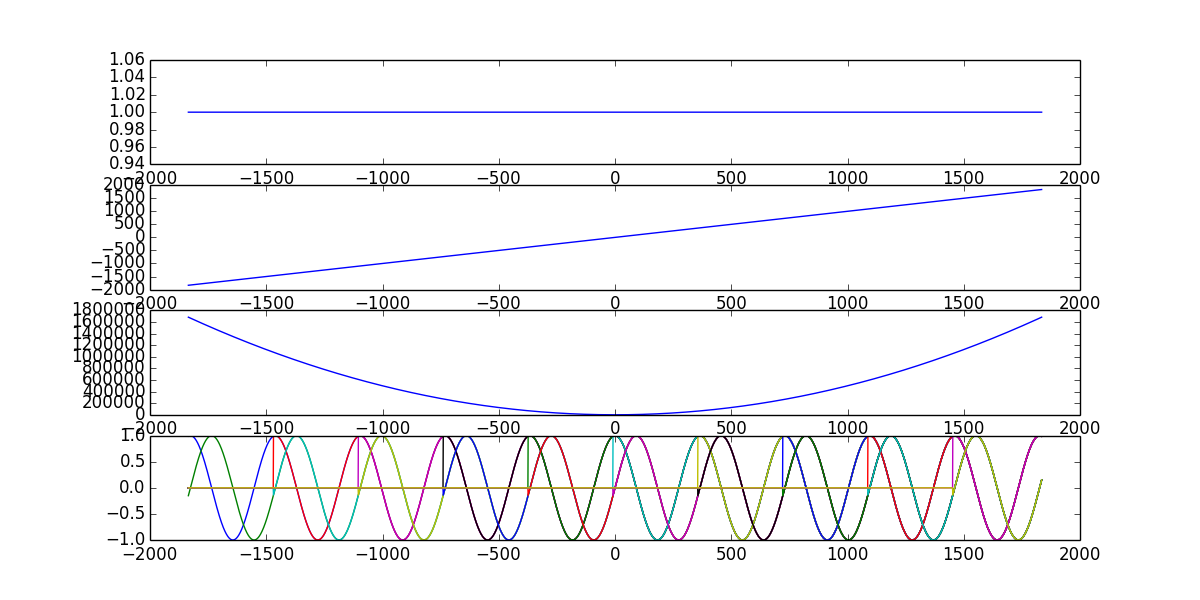
\includegraphics[width=\textwidth]{figures/splines}
	\caption{Constant, trend and acceleration in the 3 uppermost plots. Sine/cosine hinge functions in the bottom plot.}
	\label{fig:splines}
\end{figure}

Now unfortunately, although some locations gets better residuals, the resulting fits display cusps and overfitting behavior for a large proportion of the locations.
 Below follows an example of one such case

\begin{figure}[H]
	\centering
	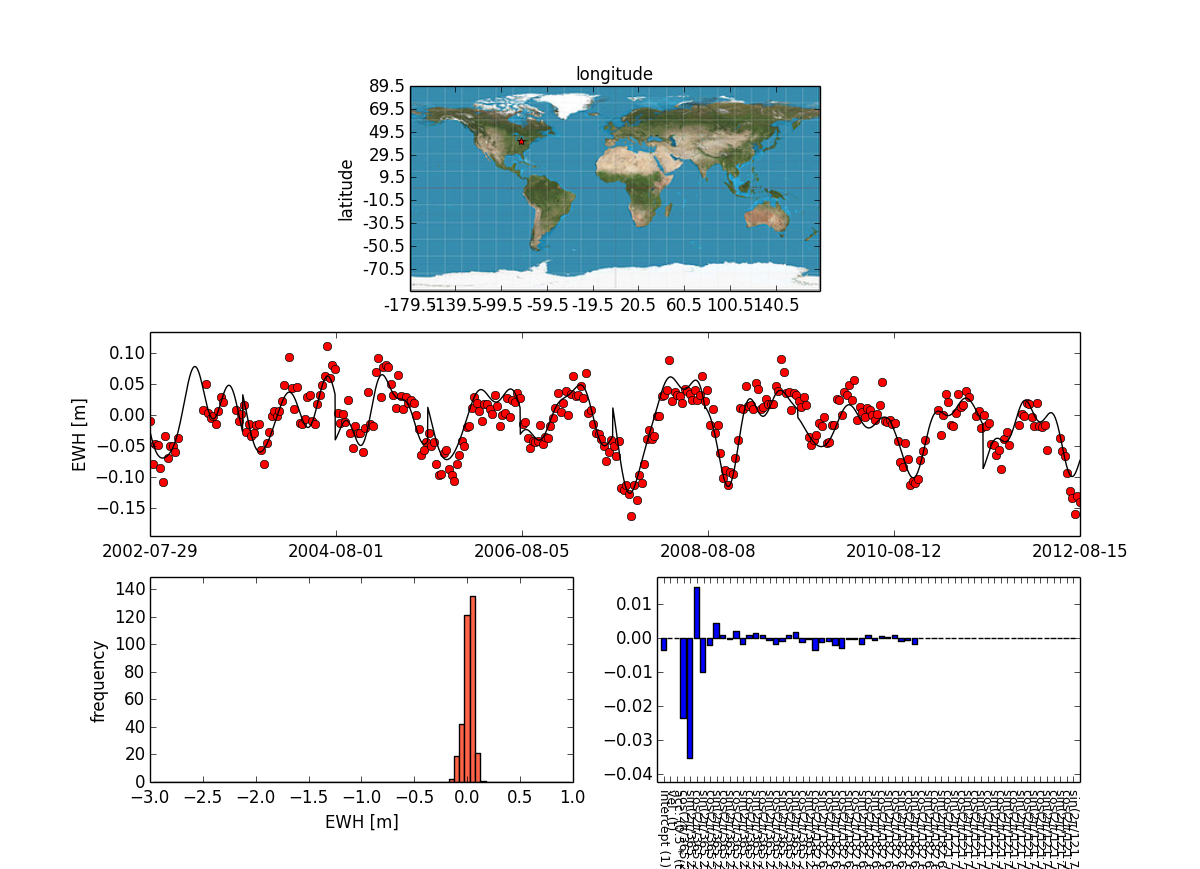
\includegraphics[width=\textwidth]{figures/res_splines_bad}
	\caption{Example of cusps and overfitting}
	\label{fig:res_splines}
\end{figure}

The above model is clearly not a valid model.
With the goal of improving on the continuity and gain spline-like characteristics attempts were made to create a new form for hinge functions.
 It was tried to generate an interval centered for each knot and then make a polynomial transition in the interval between the hinge function values at the interval endpoints.
 Although continuity was gained the resulting fit sadly looked even worse and thus it has been chosen to abstain from showing these efforts.
 \\
\subsubsection{Ideas}
If one wanted to delve deeper into the possibilities of basis expansions and hinge function the most important thing would be to analyse where to place the knots. Even though it was here chosen to place the knots at predetermined points in time and have the knots be equal for all locations, several libraries have been developed which optimizes knot location as well polynomial degrees etc.
 A famous algorithm MARS\textregistered (multivariate adaptive regression splines) developed by Jerome Friedman, can achieve this using a 2-phase pass technique \cite{wiki-MARS} (forward, backward) but implementing the algorithm seemed out of scope for this report.